\documentclass{article} 
\usepackage{amsmath}
\usepackage{enumerate}
\usepackage[unicode]{hyperref}
\hypersetup{
	colorlinks,
	citecolor=black,
	filecolor=black,
	linkcolor=black,
	urlcolor=blue
}
\usepackage[top=2cm, bottom=2cm, left = 3cm, right = 2cm]{geometry}
\usepackage{graphicx}
\usepackage{multirow}
\usepackage{textcase}
\usepackage[utf8]{vietnam}
\usepackage{booktabs}
\usepackage{adjustbox}
\usepackage{listings}
\usepackage{color}
\usepackage{ dsfont }
\usepackage{makeidx}
\usepackage[table,xcdraw]{xcolor}
% \makeindex
% \definecolor{dkgreen}{rgb}{0,0.6,0}
% \definecolor{gray}{rgb}{0.5,0.5,0.5}
% \definecolor{mauve}{rgb}{0.58,0,0.82}

% \lstset{frame=tb,
%   language=Java,
%   aboveskip=3mm,
%   belowskip=3mm,
%   showstringspaces=false,
%   columns=flexible,
%   basicstyle={\small\ttfamily},
%   numbers=none,
%   numberstyle=\tiny\color{gray},
%   keywordstyle=\color{blue},
%   commentstyle=\color{dkgreen},
%   stringstyle=\color{mauve},
%   breaklines=true,
%   breakatwhitespace=true,
%   tabsize=3
% }
% \lstset
% {language=Python}
\title{KMeans} 
\author{Nguyễn Văn Huy \& Lê Duy An} 
\begin{document}
\maketitle{} 
\newpage
\tableofcontents
\newpage

\section{Giới thiệu} % (fold)
\label{sec:giới_thiệu}

% section giới_thiệu (end)
\section{Phân tích toán học} % (fold)
\label{sec:phân_tích_toán_học}
Với dữ liệu đầu vào của thuật toán là tập hợp các điểm dữ liệu $\mathbf{X} = [\mathbf{x}_1,\mathbf{x}_2,\mathbf{x}_3,...,\mathbf{x}_N]$ $\in \mathds{R}^{d\times N}$ với $\mathbf{x}_i$ (có $d$ phần tử) là một vector mang giá trị của mỗi điểm, $N$ là số lượng các vector và số lượng $K$ các nhóm cần phân loại từ các điểm dữ liệu đó với $K < N$ (vì số lượng nhóm cần phân loại không được lớn hơn số lượng các phần tử). Điều mà chúng ta cần phải làm là làm thế nào để xác định các điểm thuộc về nhóm nào một cách gắn kết nhất, ở đây để cho dễ gọi và tính toán thì chúng ta cho rằng $K$ nhóm cần phần loại được gọi là nhóm $1,2,3,..K$. Trong phần này chúng ta chỉ đề cập đến bài toán chỉ có một điểm dữ liệu thuộc vào một nhóm duy nhất.
\\
Ban đầu chúng ta phải có được các điểm gốc ban đầu của các nhóm có thể chọn $k$ điểm bất kì hoặc có thể lấy các điểm dữ liệu có sẵn trong tập dữ liệu ban đầu. Gọi các điểm gốc ban đầu là $\mathbf{m} = [\mathbf{m}_1,\mathbf{m}_2,\mathbf{m}_3,...,\mathbf{m}_K]$ với mỗi điểm $\mathbf{m}_k$ cũng có có $d$ các giá trị tương tự như các điểm dữ liệu $\mathbf{x}_i$. Dựa vào tập các điểm gốc $\mathbf{m}_k$ chúng ta phải xác định xem điểm $\mathbf{x}_i$ thuộc vào nhóm nào và gán nhãn cho các điểm đó bằng vector $\mathbf{y}$ trong đó $\mathbf{y}_{ij} = 0$ và $\mathbf{y}_{ik} = 1$, nghĩa là vector $\mathbf{y}$ có $K$ giá trị và vị trí ở vị trí $k$ có giá trị bằng 1 thì đồng nghĩa là vector $\mathbf{x}_i$ được gán vào nhóm $k$.

% section phân_tích_toán_học (end)
\newpage
\section{Ưu và nhược điểm.} % (fold)
\label{sec:ưu_và_nhược_điểm_}
\subsection{Ưu điểm}
\begin{itemize}
	\item Thuật toán đơn giản, hiệu quả
	\item Sử dụng được với bộ số liệu lớn
\end{itemize}
\subsection{Khuyết điểm}
\begin{itemize}
	\item Cần phải xác định trước số lượng cluster. Trong thực tế, cần phải sử dụng thêm một số biện pháp giúp xác định giá trị K, chẳng hạn như elbow method.
	\item Thuật toán KMeans không đảm bảo tìm được nghiệm tối ưu toàn cục nên nghiệm cuối cùng phụ thuộc rất nhiều vào các centroid ban đầu.\\
	\begin{figure}[h]
		\centering
		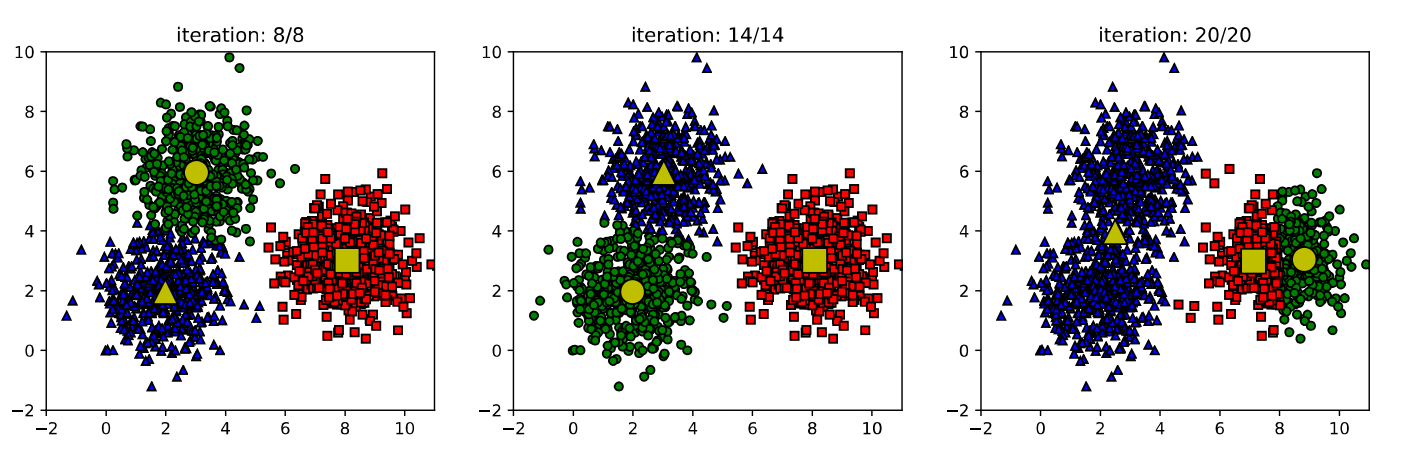
\includegraphics[width=0.7\linewidth]{img/disad_1}
		\caption{Các nghiệm khác nhau do khởi tạo ban đầu khác nhau}
	\end{figure}
	\item Các cluster cần phải có số lượng điểm gần bằng nhau\\
	\begin{figure}[h]
		\centering
		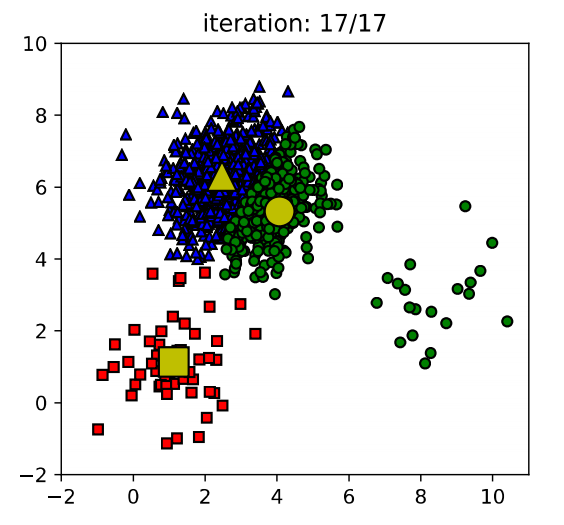
\includegraphics[width=0.3\linewidth]{img/disad_2}
		\caption{Các nghiệm trong cluster này bị nhầm vào cluster khác}
	\end{figure}
	\item Các cluster cần có dạng hình tròn (cầu)	
	\begin{figure}[h]
		\centering
		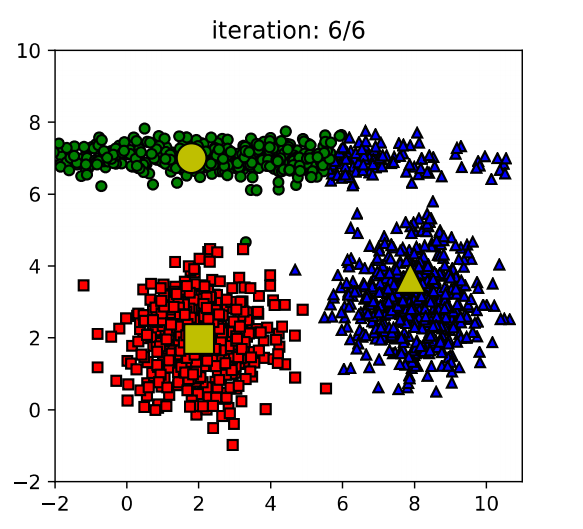
\includegraphics[width=0.3\linewidth]{img/disad_3}
		\caption{Các nghiệm trong cluster này bị nhầm vào cluster khác}
	\end{figure}
	\item Centroid có thể bị xê dịch bởi các ngoại lệ, hoặc các ngoại lệ có thể có cụm riêng thay vì bị bỏ qua.
	\item Cho kết quả sai khi một cluster này bị bao bọc bằng một cluster khác
	\begin{figure}[h]
		\centering
		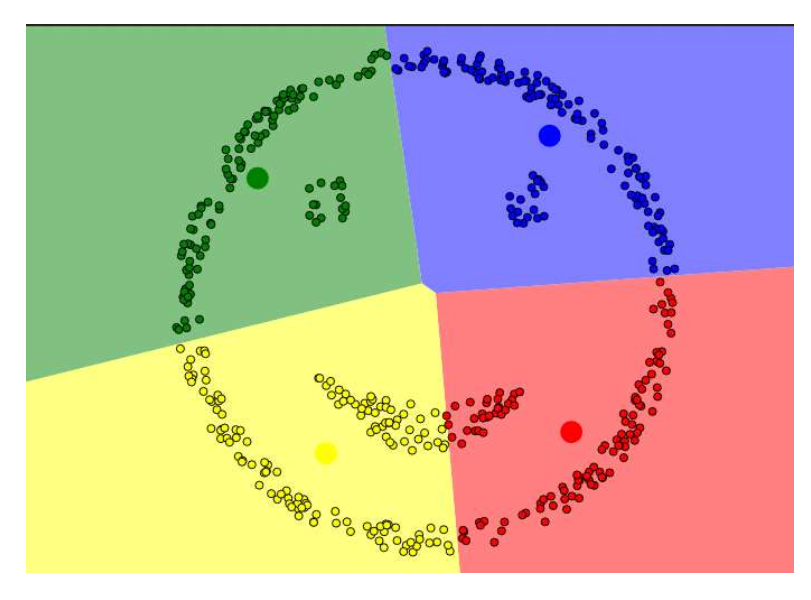
\includegraphics[width=0.7\linewidth]{img/disad_4}
		\caption{KMeans chia mặt làm 4 phần thay vì gom chung các bộ phận trong khuôn mặt thành 1 cụm}
	\end{figure}	
\end{itemize}
\newpage

\newpage
\section{Cách tìm K cụm tối ưu nhất}

% section cách_tìm_k_cụm_tốt_nhất (end)
\end{document}
